%%%%%%%%%%%%%%%%%%%%%%%%%%%%%%%%%%%%%%%%%%%%%%%%%%%%%%%%%
%Este documento representa la plantilla de los articulos%
%a ser editados para la revista, realizada bajo codigo  %
%        Latex, con una clase ``article``               %   
%          PUBLICACIONES EN CIENCIAS                    %               
%                Y  TECNOLOGIA.                         %
%        Realizado por Adriana Araujo                   %
%       Revisado por Hugo Lara              (2014)      %        
%              Cuerpo editorial.                        %
%%%%%%%%%%%%%%%%%%%%%%%%%%%%%%%%%%%%%%%%%%%%%%%%%%%%%%%%%
\documentclass[11pt,twoside,A5]{article}
\usepackage[spanish]{babel}
\usepackage[utf8]{inputenc}
\usepackage{amsmath}
\usepackage{amsfonts}
\usepackage{amssymb}
\usepackage{amscd}
\usepackage{psfrag}
\usepackage{graphicx}
%%%%%%%%%%%%%%%%%%%%%%%%%%%%%%%%%%
%\theoremstyle{theorem}
\newtheorem{thm}{Theorem}[section]
\newtheorem{prop}{Proposition}[section]
\newtheorem{clly}{Corollary}[section]
\newtheorem{lem}{Lemma}[section]
\newtheorem{pf}{Proof}[section]
%\theoremstyle{definition}
\newtheorem{defi}{Definition}[section]
\newtheorem{exam}{Example}[section]
\newtheorem{rk}{Remark}[section]
\def\proof{\mbox {\it Proof.~}}
\newcommand{\en}{\~n}
\newcommand{\figura}{\stepcounter{figure}}
\newcommand{\cuadro}{\stepcounter{table}}
\renewcommand{\tablename}{Tabla}
\newtheorem{pot}{Proof of Theorem} %\ref{mainthm}}
%%%%%%%%%%%%%%%%%%%%%%%%%%%%%%%%%%%%%%%%%%
\def\N{\mathbb{N}}
\def\Z{\mathbb{Z}}
\def\Q{\mathbb{Q}}
\def\R{\mathbb{R}}
\def\C{\mathbb{C}}
\def\K{\mathbb{K}}
\def\V{\mathbb{V}}
\def\U{\mathbb{U}}
\def\O{\mathcal{O}}
\def\A{\mathcal{A}}
\def\L{\mathcal{L}}
\def\Rc{\mathcal{R}}
\newcommand{\vect}{\overrightarrow}
\newcommand{\modN}{\;\text{(mod $N$)}}

\usepackage[pass,paperwidth=15cm,paperheight=22cm]{geometry}
\paperheight=22cm
  \paperwidth=15cm
\setlength{\oddsidemargin}{-0.5cm} \setlength{\evensidemargin}{-1.0cm}
\setlength{\topmargin}{-1.5cm} \setlength{\textwidth}{11.5cm}
\setlength{\textheight}{17.5cm}


\setcounter{page}{1}
%%%%%%%%%%%%%%%%%%%%%%%%%%%%%%%%%%

%%%%%%%%%%%%%%%%%%%%%%%%%%%%%%%%%%%%%%%
\usepackage{fancyhdr}
\pagestyle{fancy}
%%%%%%%%%%%%%%%%%%%%%%%%%%%%%%%%%%%%%%%%%%%%%%%%%%%%%%%%%%%%%%%%%%%%%%%%%%%%%%%%%%%%%%%%%%%%%%%%%%%%%%%%%%%%%%%
%%%%%%%%SECCION DEL TITULO Y TIRILLA BIBLIOGRAFICA(ESTA ULTIMA PARA USO INTERNO DEL CUERPO EDITORIAL)%%%%%%%%%%
%%%%%%%%%%%%%%%%%%%%%%%%%%%%%%%%%%%%%%%%%%%%%%%%%%%%%%%%%%%%%%%%%%%%%%%%%%%%%%%%%%%%%%%%%%%%%%%%%%%%%%%%%%%%%%%
\begin{document}
\title{
\vspace{-1.1in}
\begin{flushleft}
{\normalsize \begin{center}
%{\em\bf Publicaciones en Ciencias y Tecnolog\'ia}\\ 
%\scriptsize{Vol 7, N$^{0}$2, Jul--Dic 2013, pp.7--15,   ISSN:1856-8890, Dep\'osito Legal:pp200702LA2730 }
%\small{Art\'iculo en revisi\'on.  ISSN:1856-8890, Dep\'osito Legal: pp200702LA2730}
\end{center}}
\end{flushleft}
\hrule \vspace{0.5in}{ARQUITECTURA DE NAVEGACIÓN HÍBRIDA PARA ROBOT PIONEER PD3X} }
%%%%%%%%%%%%%%%%%%%%%%%%%%%%%%%%%%%%%%%%%%%%%%%%%%%%%%%%%%%%%%%%%%%%%%%%%%%%%%%%%%%%%%%%%%%%%%%%%%%%%%%%%%%%%%%
%%%%%%%%SECCION AUTORES Y FILIACION DE LOS MISMOS %%%%%%%%%%%%%%%%%%%%%%%%%%%%%%%%%%%%%%%%%%%%%%%%%%%%%%%%%%%%%%
%%%%%%%%%%%%%%%%%%%%%%%%%%%%%%%%%%%%%%%%%%%%%%%%%%%%%%%%%%%%%%%%%%%%%%%%%%%%%%%%%%%%%%%%%%%%%%%%%%%%%%%%%%%%%%%

\author{ 
\footnote{  {\it\scriptsize  Decanato de Ciencias y Tecnolog\'ia,} 
{\it\scriptsize Universidad Centroccidental Lisandro Alvarado,}
{\it\scriptsize Barquisimeto, Venezuela, sauljabin@gmail.com}
}\hspace{1mm}{Saúl Piña}
 \hspace{3mm} 
\footnote{  {\it\scriptsize  Decanato de Ciencias y Tecnolog\'ia,} 
{\it\scriptsize Universidad Centroccidental Lisandro Alvarado,}
{\it\scriptsize Barquisimeto, Venezuela, thejorgemylio@gmail.com}
}\hspace{1mm}{ Jorge Parra} \\
 %\hspace{3mm} 
%\footnote{  {\it\scriptsize Departamento-Instituto-Facultad}, 
%{\it\scriptsize Universidad-Instituci\'on (filiaci\'on)},
%{\it\scriptsize Lugar, Pa\'is, email}
%}\hspace{5mm}{ Nombre autor 3 }
% \hspace{3mm} 
%\hspace{3mm}
%\footnote{ {\it\scriptsize  Departamento de Ingenier\'ia Industrial,  Instituto Tecnol\'ogico de Celaya}, 
%{\it\scriptsize Instituto Tecnol\'ogico de Celaya},  
%{\it\scriptsize M\'exico, gesparza@itc.mx }
%}\hspace{5mm} { Luis Gerardo Esparza-D\'iaz}
}

%\vspace{-15mm}
\date{\small{Octubre 2014}
}

%\date{}
%%%%%%%%%%%%%%%%%%%%%%%%%%%%%%%%%%
\maketitle 
%%%%%%%%%%%%%%%%%%%%%%%%%%%%%%%%%%%%%%%%%%%%%%%%%%%%%%%%%%%%%%%%%%%%%%%%%%
% SECCION TITULO CORTO E INICIALES AUTORES, HASTA DOS AUTORES:
% APELLIDO 1, INICIAL NOMBRE 1. ; APELLIDO 2, INICIAL NOMBRE 2.
%                        MAS DE DOS 
%                APELLIDO, INICIAL NOMBRE. et al
%%%%%%%%%%%%%%%%%%%%%%%%%%%%%%%%%%%%%%%%%%%%%%%%%%%%%%%%%%%%%%%%%%%%%%%%%%%
\fancyhead{} \fancyhead[CE]{ ARQUITECTURA DE NAVEGACIÓN HÍBRIDA PARA ROBOT PIONEER PD3X  }
\fancyhead[CO]{ Saúl Piña, Jorge Parra 
}
\fancyfoot{}
%\fancyfoot[CO,CE]{\scriptsize{{Publicaciones en Ciencias y Tecnolog\'ia.} Vol 7,N$^{0}$2, Jul--Dic 2013, pp.07--15.}}
%\fancyfoot[CO,CE]{Publicaciones en Ciencias y Tecnolog\'ia. Art\'iculo en revisi\'on}
\fancyfoot[RO,LE]{\thepage}

%%%%%%%%%%%%%%%%%%%%%%%%%%%%%%%%%%%%%%%%%%%%%%%%%%%%%%%%%%%%%%%%%%%%%%%%%%%%%
%%%%%%%%%%%%%%%%%%SECCION DE RESUMEN Y ABSTRACT%%%%%%%%%%%%%%%%%%%%%%%%%%%%%%
%%%%%%%%%%%%%%%%%%%%%%%%%%%%%%%%%%%%%%%%%%%%%%%%%%%%%%%%%%%%%%%%%%%%%%%%%%%%%
\begin{center}
{\bf\small Resumen}
%\vspace{-5mm}

\vspace{-3mm} \hspace{.05in}\parbox{4.5in} {{\small %\footnotesize 

Cuerpo del resumen (Max 200 palabras)

 \textbf{Palabras clave}: Robótica, ARIA, AuRA, Arquitectura Híbrida, Pioneer P3DX}}
\end{center}
\pagebreak


\begin{center}
{\bf\small T\'ITULO EN INGL\'ES \\ Abstract}

\vspace{-3mm} \hspace{.05in}\parbox{4.5in} {{\small %\footnotesize 

Cuerpo del abstract  

     \textbf{Keywords}:  kw 1, kw 2, ... .}}
\end{center}
%%%%%%%%%%%%%%%%%%%%%%%%%%%%%%%%%%%%%%%%%%%%%%%%%%%%%%%%%%%%%%%%%%%%%%%%%%%%%%%%%%%%%%%
%                           CUERPO DEL ARTICULO
%%%%%%%%%%%%%%%%%%%%%%%%%%%%%%%%%%%%%%%%%%%%%%%%%%%%%%%%%%%%%%%%%%%%%%%%%%%%%%%%%%%%%%%
%\pagebreak

\section*{Introducción }

\section*{Pioneer P3DX}

\begin{figure}[here]
\begin{center}
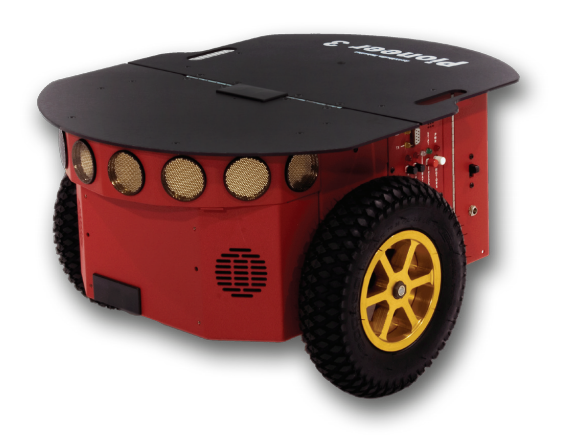
\includegraphics[width=6cm]{pioneer.png} 
\caption{Robot Pioneer P3DX}
\label{fig:pioneer}
\end{center}
\end{figure} 

\section*{Arquitectura AuRA}

Explicar AuRA

\section*{Implementación de la Arquitectura}

Explicar como se programo el Aura

\section*{Entorno de Desarrollo}

La herramienta desarrollada 

Explicar las herramientas usadas, aria, mobilesim, eclipse, java, windows

\section*{Configuración del Entorno}

La herramienta de software se creo usando tecnología multiplataforma, por ende 
el entorno de desarrollo se puede configurar en sistemas operativos Windows o Linux.



Instrucciones para instalar todo \url{https://bitbucket.org/sauljabin/ariajava-p3dx}

\section*{Herramienta de Software Desarrollada}



\section*{Experimentación}

Explicar los experimentos realizados

%%%%%%%%%%%%%%%%%%%%%%%%%%%%%%%%%%%%%%%%%%%%%%%%%%%%%%%%%%%%%%%%%%%%%%%%%%%%%%%%%%%%%%%%
%                                 BIBLIOGRAFIA
%%%%%%%%%%%%%%%%%%%%%%%%%%%%%%%%%%%%%%%%%%%%%%%%%%%%%%%%%%%%%%%%%%%%%%%%%%%%%%%%%%%%%%%%
\begin{thebibliography}{999}

\end{thebibliography}
\end{document}
